\chapter{Υλοποίηση εφαρμογής} \label{ch:unitask}
    Σε αυτό το κεφάλαιο...

    \section{Σχεδίαση}
        Στην ενότητα \ref{sec:student_preferences}, παρουσιάστηκε μια έρευνα με τα βασικά χαρακτηριστικά που θεωρήθηκαν απαραίτητα από τους φοιτητές για μια εφαρμογή τους. Λαμβάνοντας υπόψιν τις προτιμήσεις αυτές δόθηκε βάση στην υλοποίηση τους ώστε η εφαρμογή να ανταποκρίνεται στις ανάγκες της ακαδημαϊκής κοινότητας.

        Αρχικά, ως μια εφαρμογή διαχείρισης εργασιών, θα περιλαμβάνει προφανώς ένα σύστημα δημιουργίας, τροποποίησης και διαγραφής εργασιών, καθορισμού του χρόνου έναρξης και λήξεώς τους, και η κατηγοροποίηση των εργασιών σε κατηγορίες ανάλογα με το αν έχουν πραγματοποιηθεί, αν πραγματοποιούνται και αν έχουν σκοπό να πραγματοποιηθούν μελλοντικά. Επιπλέον, με βάση την έρευνα, είναι σημαντική η ενσωμάτωση ενός ημερολογίου, η δυνατότητα χρωματικής ταξινόμησης (color-coding) και η υλοποίηση ενός συστήματος ανταμοιβής για την ενίσχυση της παρακίνησης των χρηστών. Επίσης, θα ήταν εξίσου σημαντική η δημιουργία ενός Kanban πίνακα για την άμεση οπτικοποίηση των εργασιών και την ευκολότερη διαχείρισή τους.

        Σχεδιαστικά θεωρείται σημαντική η τήρηση σύγχρονων σχεδιαστικών κανόνων με ένα καθαρό interface και συνοχή στο σχεδιασμό για τη δημιουργία μιας λειτουργικής, αισθητικά ευχάριστης και ευκολόχρηστης εμπειρίας χρήστη ώστε να εξασφαλιστεί ότι η εφαρμογή μπορεί να ανταποκριθεί στις ανάγκες διαφορετικών τύπων χρηστών, αλλά και να παρουσιαστεί ως ένα προϊόν έτοιμο για χρήση σε πραγματικά περιβάλλοντα.

        Στα σχήματα \ref{fig:unitaskMockupCalendar}, \ref{fig:unitaskMockupDashboard} και \ref{fig:unitaskMockupKanban} παρουσιάζονται κάποια αρχικά mockups που χρησιμοποιήθηκαν για το σχεδιασμό της εφαρμογής.

        \begin{figure}[h!] \noindent \centering
            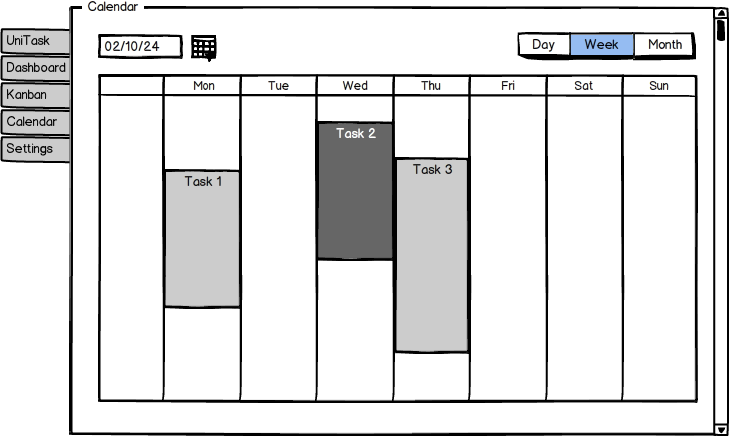
\includegraphics[width=0.65\textwidth]{mockups/Calendar}
            \caption{\centering Mockup Calendar σελίδας}
            \label{fig:unitaskMockupCalendar}
        \end{figure}

        \begin{figure}[h!] \noindent \centering
            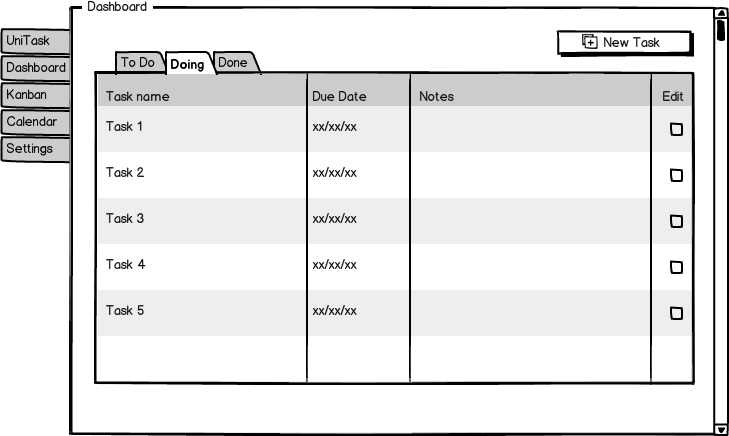
\includegraphics[width=0.65\textwidth]{mockups/Dashboard}
            \caption{\centering Mockup Dashboard σελίδας}
            \label{fig:unitaskMockupDashboard}
        \end{figure}

        \begin{figure}[h!] \noindent \centering
            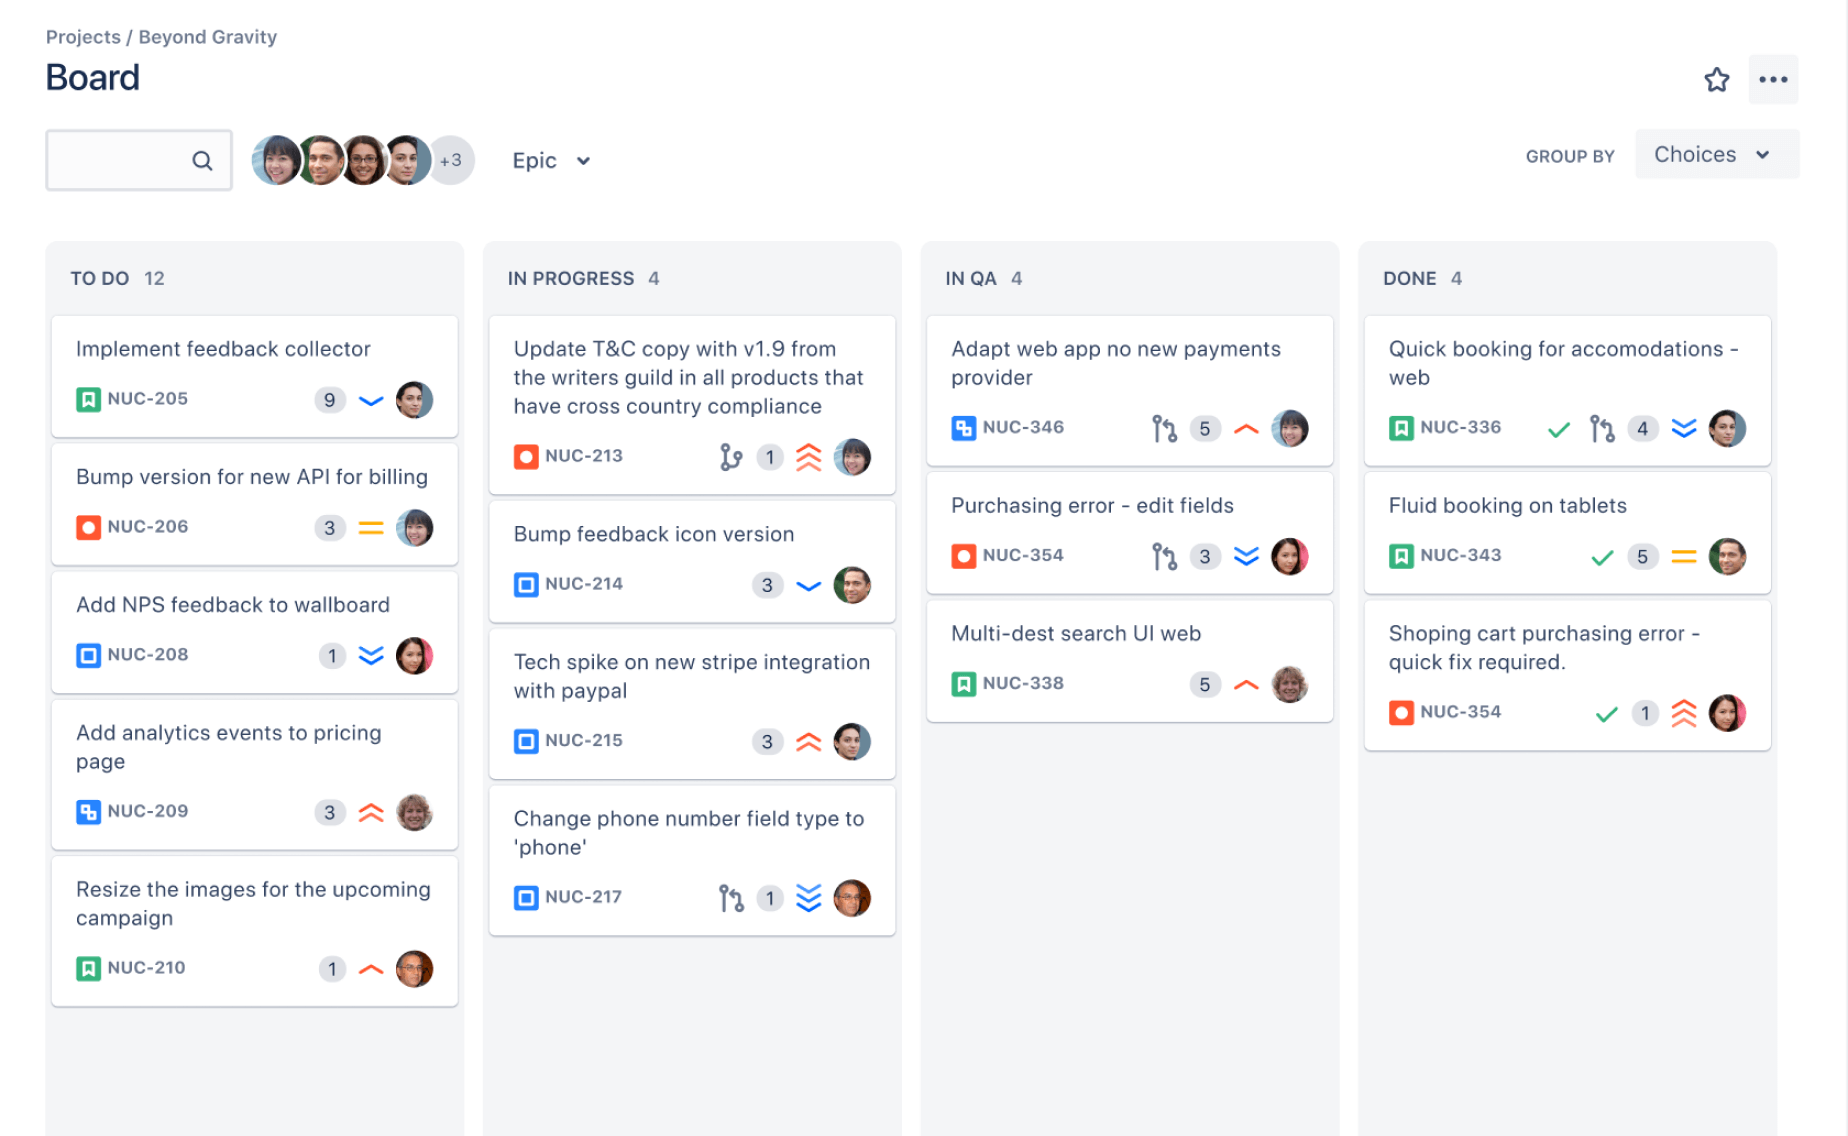
\includegraphics[width=0.65\textwidth]{mockups/Kanban}
            \caption{\centering Mockup Kanban σελίδας}
            \label{fig:unitaskMockupKanban}
        \end{figure}

    \pagebreak

    \section{Η εφαρμογή}
        Κατά την εκτέλεση της εφαρμογής, είτε τοπικά είτε μέσω της απομακρυσμένης πρόσβασης στο cloud, στη διεύθυνση \texttt{https://unitask-sandbox.mxapps.io/}, εμφανίζεται αρχικά η \textbf{σελίδα σύνδεσης}, όπως φαίνεται στο σχήμα \ref{fig:unitask_Login}. Στη συγκεκριμένη σελίδα, οι χρήστες καλούνται να εισάγουν τα στοιχεία σύνδεσής τους για να αποκτήσουν πρόσβαση στις λειτουργίες της εφαρμογής.

        Ανάλογα με τα στοιχεία σύνδεσης που παρέχονται, το σύστημα διακρίνει δύο επίπεδα πρόσβασης: δικαιώματα διαχειριστή (Administrator) και δικαιώματα χρήστη (User), όπου εκπροσωπούν τους φοιτητές. Οι χρήστες με δικαιώματα Administrator έχουν πρόσβαση σε επιπλέον προηγμένες λειτουργίες διαχείρισης όπως η διαχείριση των χρηστών.

       \begin{figure}[h!] \noindent \centering
            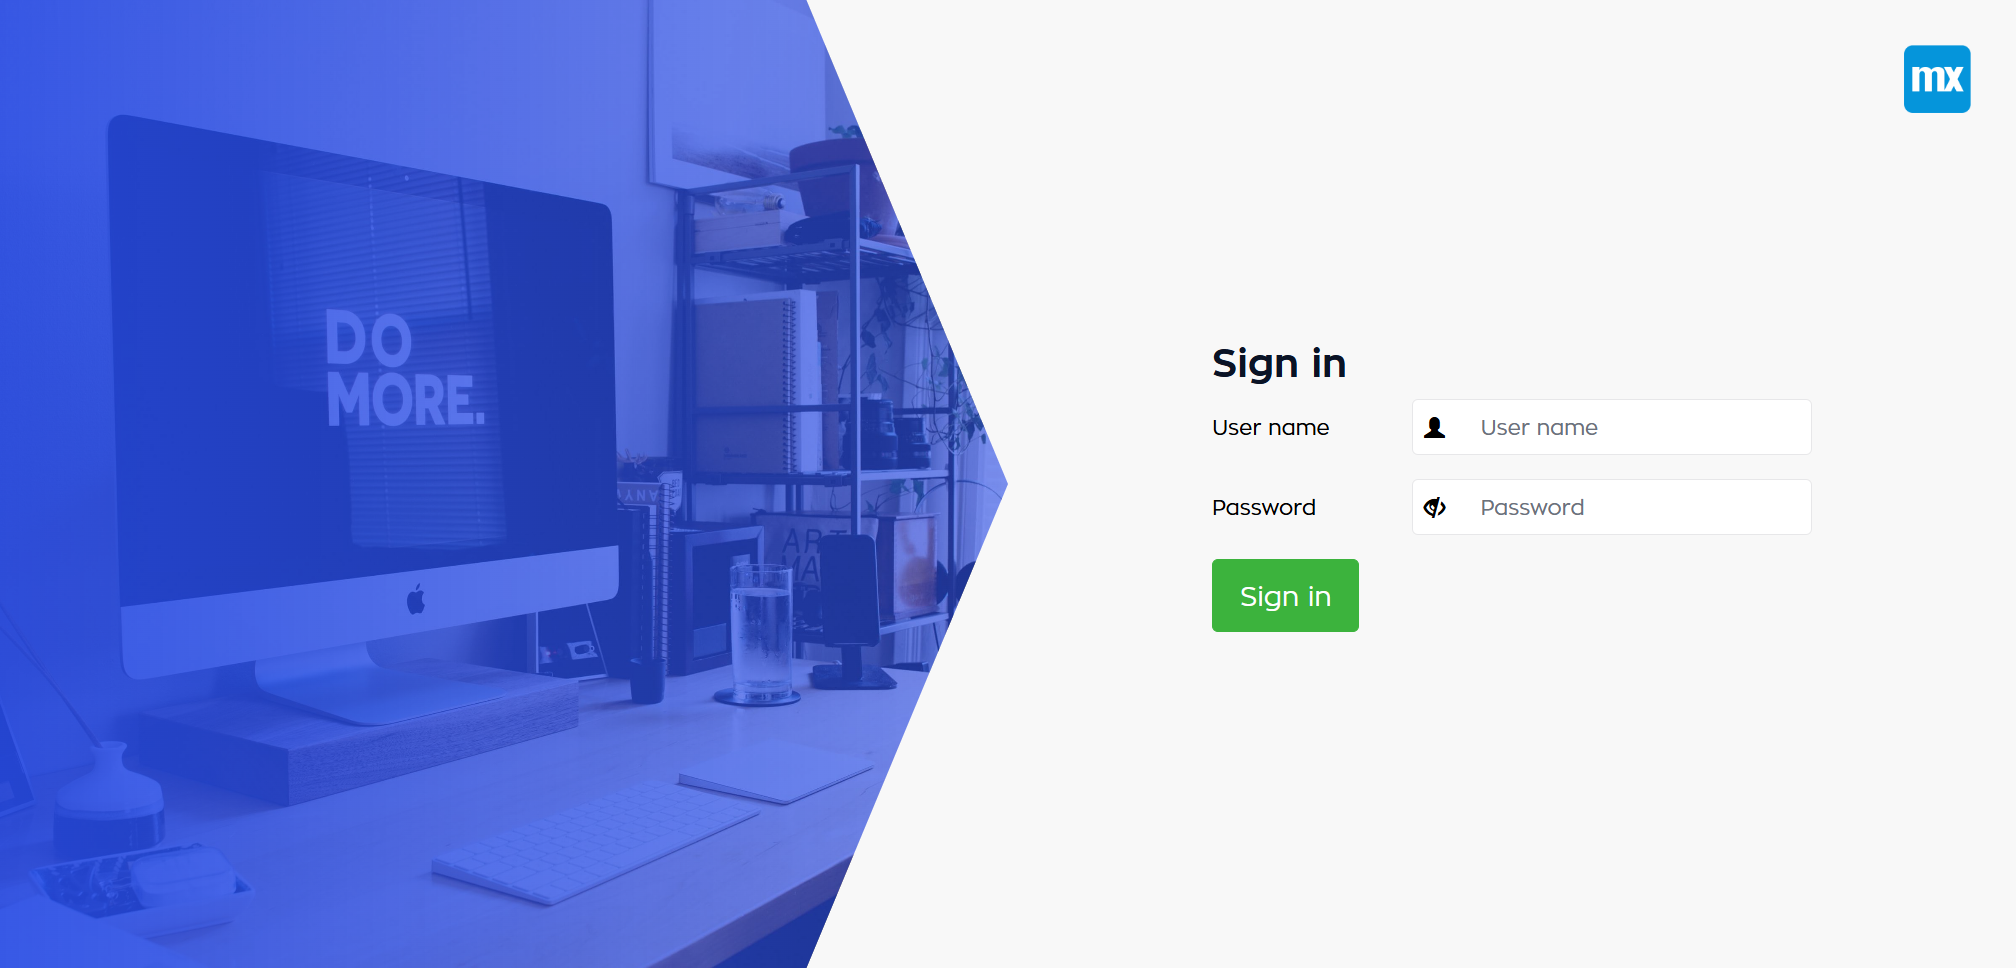
\includegraphics[width=\textwidth]{UniTask/Login}
            \caption{\centering Σελίδα σύνδεσης}
            \label{fig:unitask_Login}
        \end{figure}

        Αρχικά, πραγματοποιείται σύνδεση με τον λογαριασμό διαχειριστή (Administrator) προκειμένου να παρουσιαστούν οι λειτουργίες διαχείρισης χρηστών, συμπεριλαμβανομένης της δυνατότητας προσθήκης νέου χρήστη. Μετά την επιτυχή εισαγωγή των διαπιστευτηρίων του διαχειριστή, τα οποία έχουν οριστεί προκαταβολικά κατά την ανάπτυξη της εφαρμογής (βλ. ενότητα \ref{sec:unitask_mendix}), εμφανίζεται η \textbf{σελίδα διαχείρισης χρηστών}, όπως απεικονίζεται στο σχήμα \ref{fig:unitask_AccountOverview}. Η σελίδα αυτή παρέχει στους διαχειριστές μια ολοκληρωμένη επισκόπηση της λίστας χρηστών της εφαρμογής, καθώς και εργαλεία για τη διαχείρισή τους. Το layout της σελίδας αποτελείται από μια κάθετη μπάρα μενού η οποία περιλαμβάνει τις ίδιες δυνατότητες με τους απλούς χρήστες η οποίες θα αναλυθούν στη συνέχεια.

       \begin{figure}[h!] \noindent \centering
            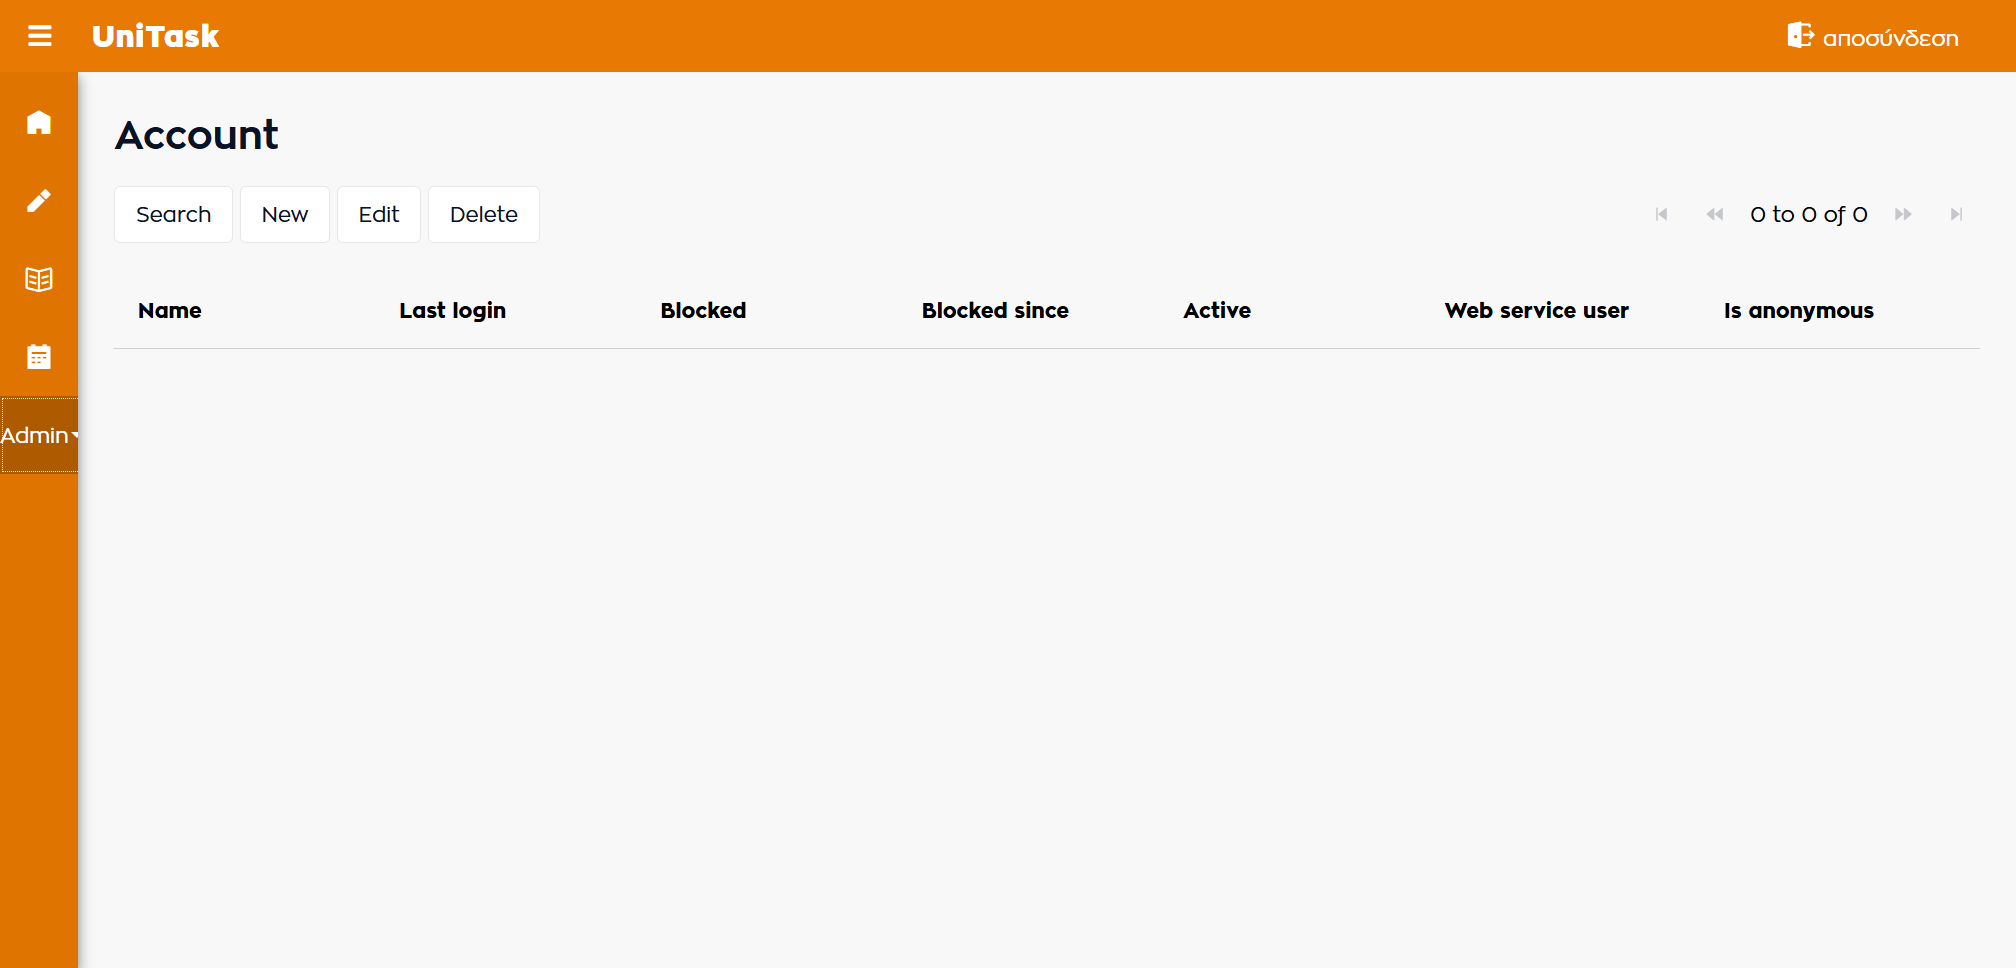
\includegraphics[trim={0 12cm 0 0}, clip, width=\textwidth]{UniTask/AccountOverview}
            \caption{\centering Σελίδα διαχείρισης χρηστών}
            \label{fig:unitask_AccountOverview}
        \end{figure}

        Πατώντας στο κουμπί {\Zona New}, εμφανίζεται η popout σελίδα του σχήματος \ref{fig:unitask_NewAccount} με μια \textbf{φόρμα για την προσθήκη νέου χρήστη}. Η φόρμα περιλαμβάνει πεδία για την εισαγωγή του ονόματος χρήστη ({\Zona Username}), του ρόλου του χρήστη ({\Zona User role}) όπου επιλέγεται αν πρόκειται για προσθήκη διαχειριστή ή χρήστη, του κωδικού πρόσβασης ({\Zona New password} και {\Zona Confirm password}). Λόγω του ότι ο χρήστης User έχει κληρονομήσει γνωρίσματα από την κλάση \texttt{System.User} του Mendix, έχουν προστεθεί πεδία όπως το {\Zona Blocked}, η οποία γίνεται αληθής μετά από κάποιες αποτυχημένες προσπάθειες σύνδεσης, το {\Zona Active} που γίνεται αληθές όταν ο χρήστης συνδεθεί, το {\Zona Time zone} όπου ορίζεται η ζώνη ώρας του χρήστη και το {\Zona Language} όπου ορίζεται η γλώσσα του χρήστη.

        \begin{figure}[h!] \noindent \centering
            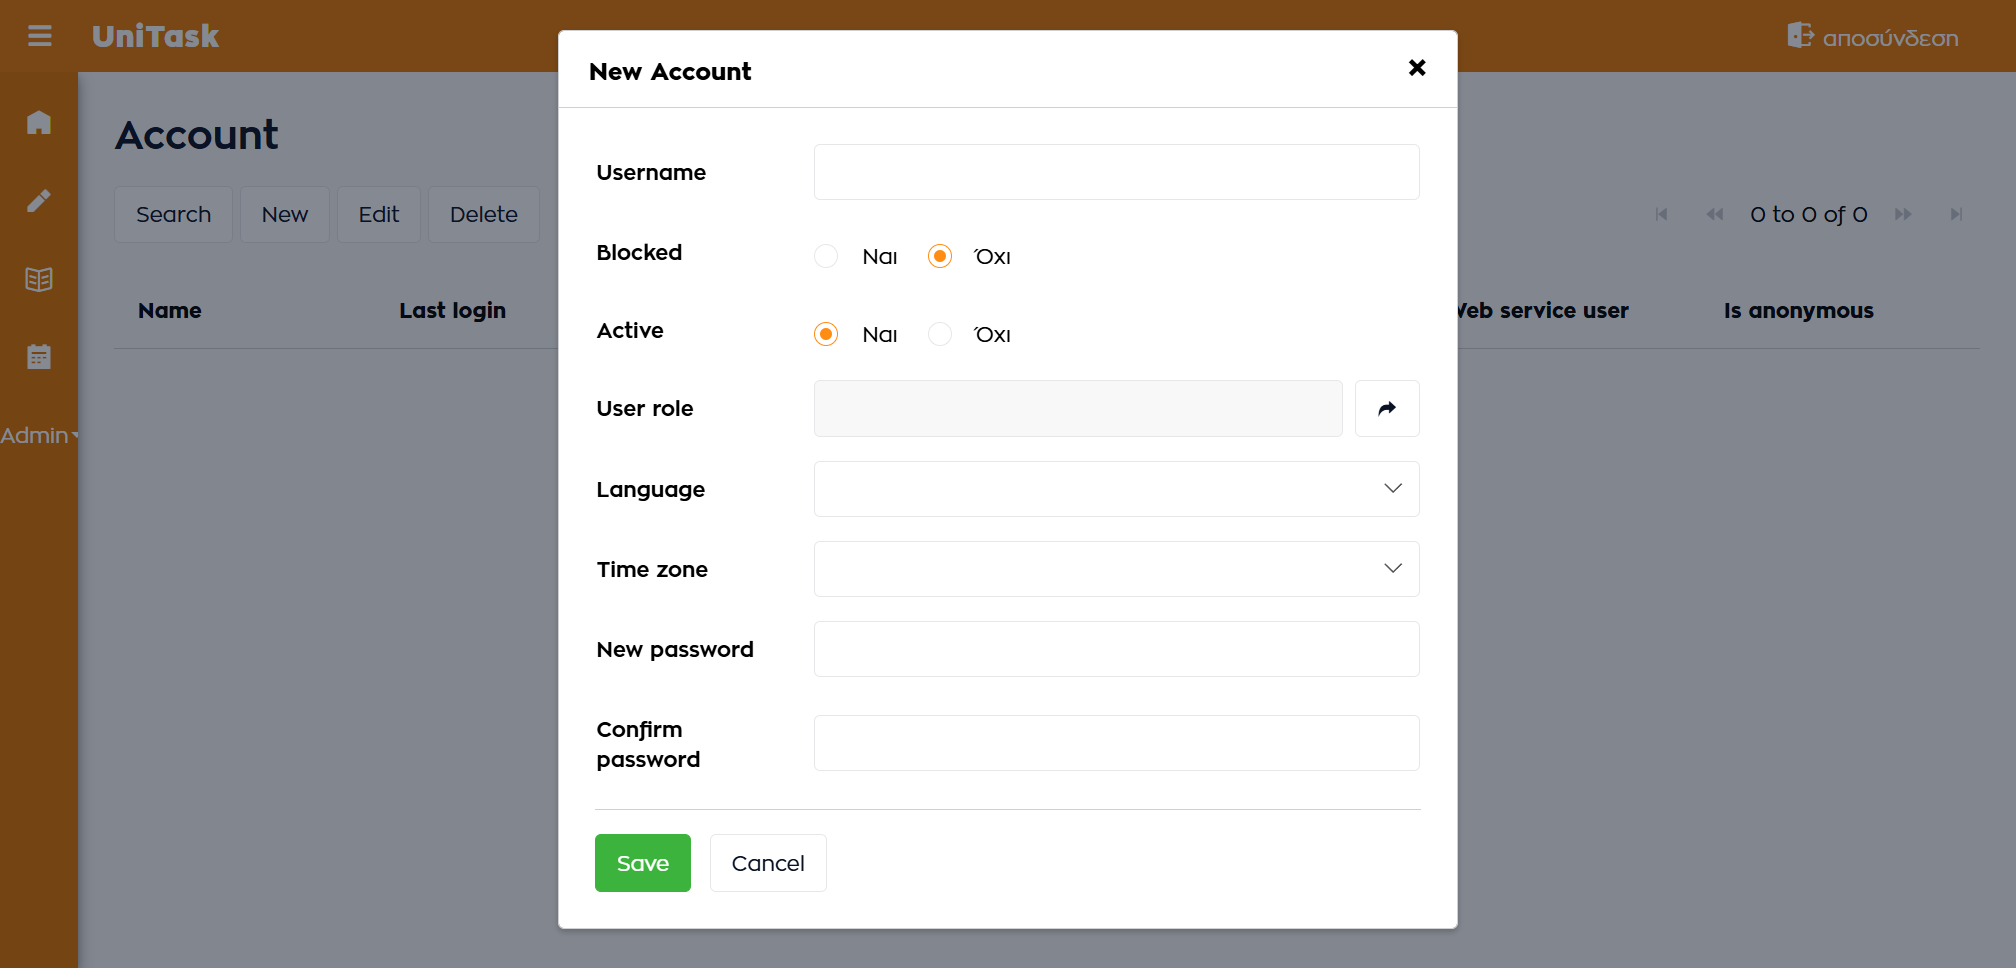
\includegraphics[width=\textwidth]{UniTask/NewAccount}
            \caption{\centering Φόρμα προσθήκης νέου χρήστη}
            \label{fig:unitask_NewAccount}
        \end{figure}

        Δημιουργούμε έναν χρήστη με όνομα \texttt{Foithths}, ο οποίος εμφανίζεται στη λίστα των χρηστών (σχήμα \ref{fig:unitask_AccountOverview_WithStudent}. Πατώντας στο όνομά του, εμφανίζεται η σελίδα επεξεργασίας του χρήστη, όπως φαίνεται στο σχήμα \ref{fig:unitask_EditAccount}. Στη λίστα των χρηστών υπάρχει η δυνατότητα αναζήτησης χρηστών βάσει όλων των στοιχείων τους (σχήμα \ref{fig:unitask_SearchAccounts}), όπως επίσης και η δυνατότητα διαγραφής τους.

        \begin{figure}[h!] \noindent \centering
            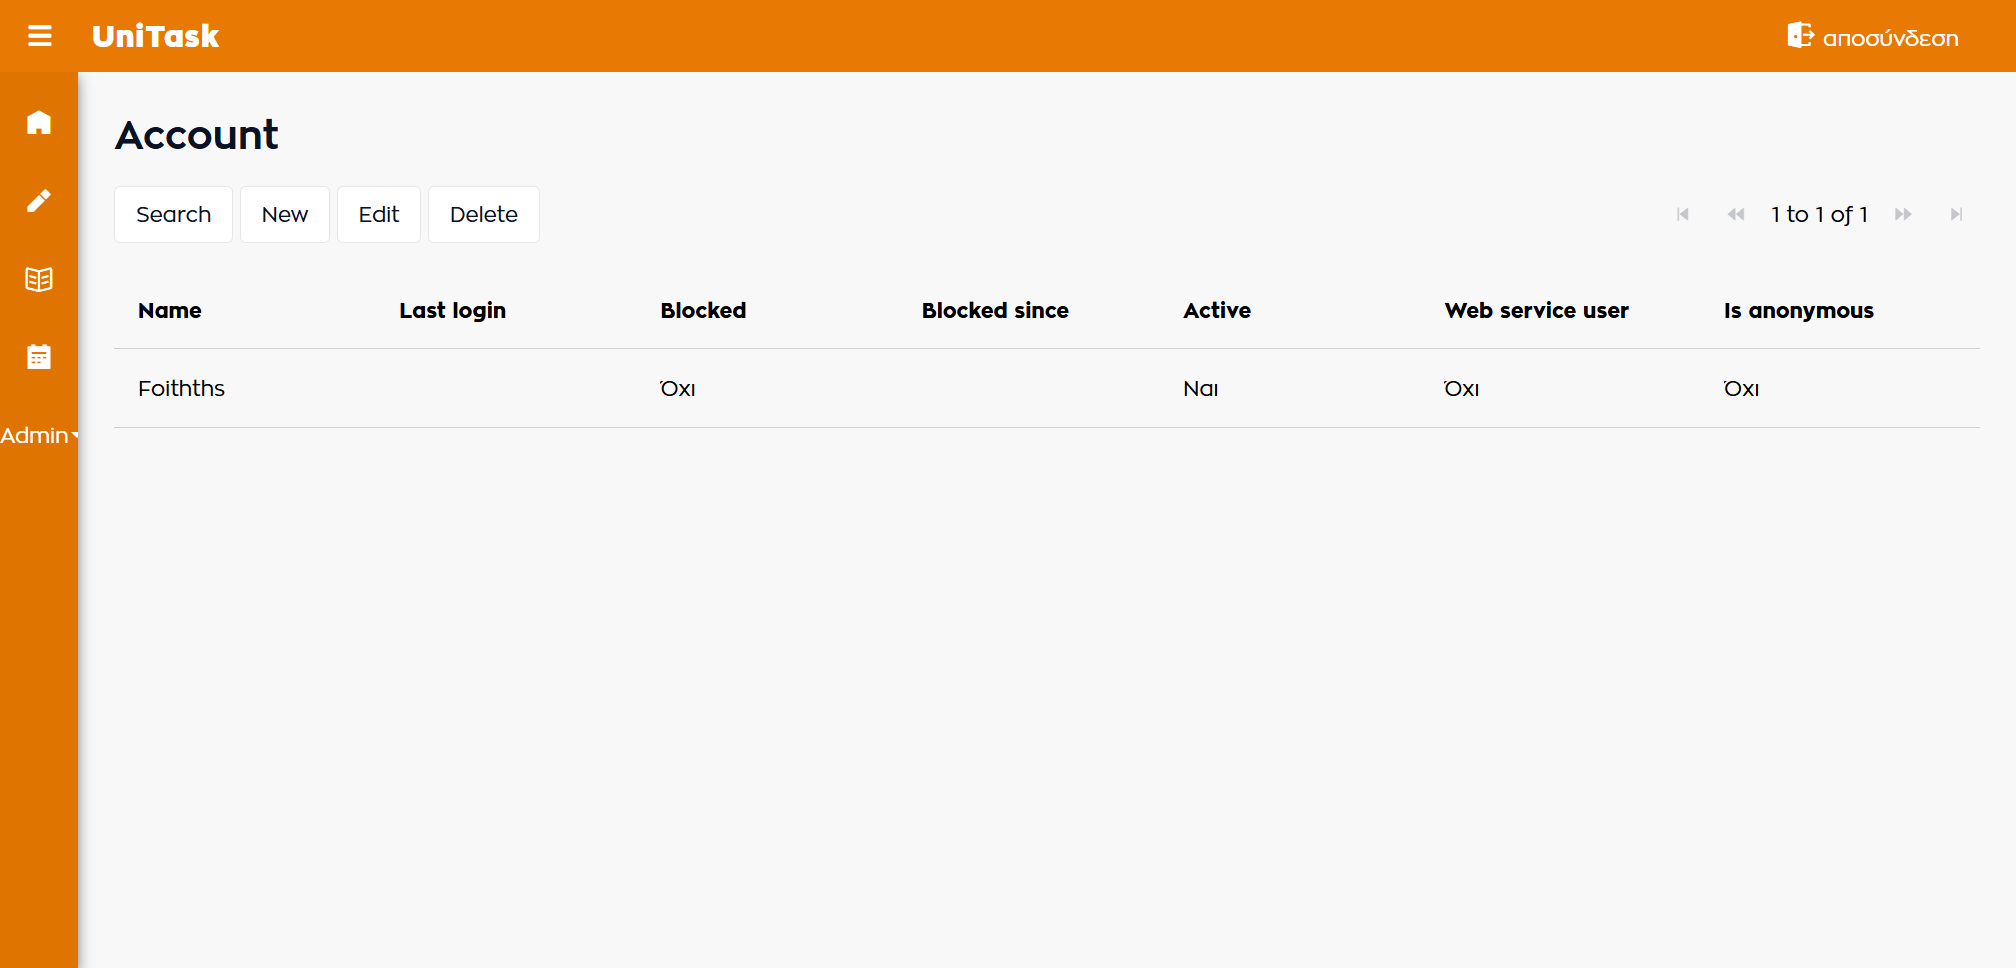
\includegraphics[trim={0 17cm 0 0}, clip, width=\textwidth]{UniTask/AccountOverview_WithStudent}
            \caption{\centering Λίστα χρηστών με τον χρήστη \texttt{Foithths}}
            \label{fig:unitask_AccountOverview_WithStudent}
        \end{figure}

        \begin{figure}[h!] \noindent \centering
            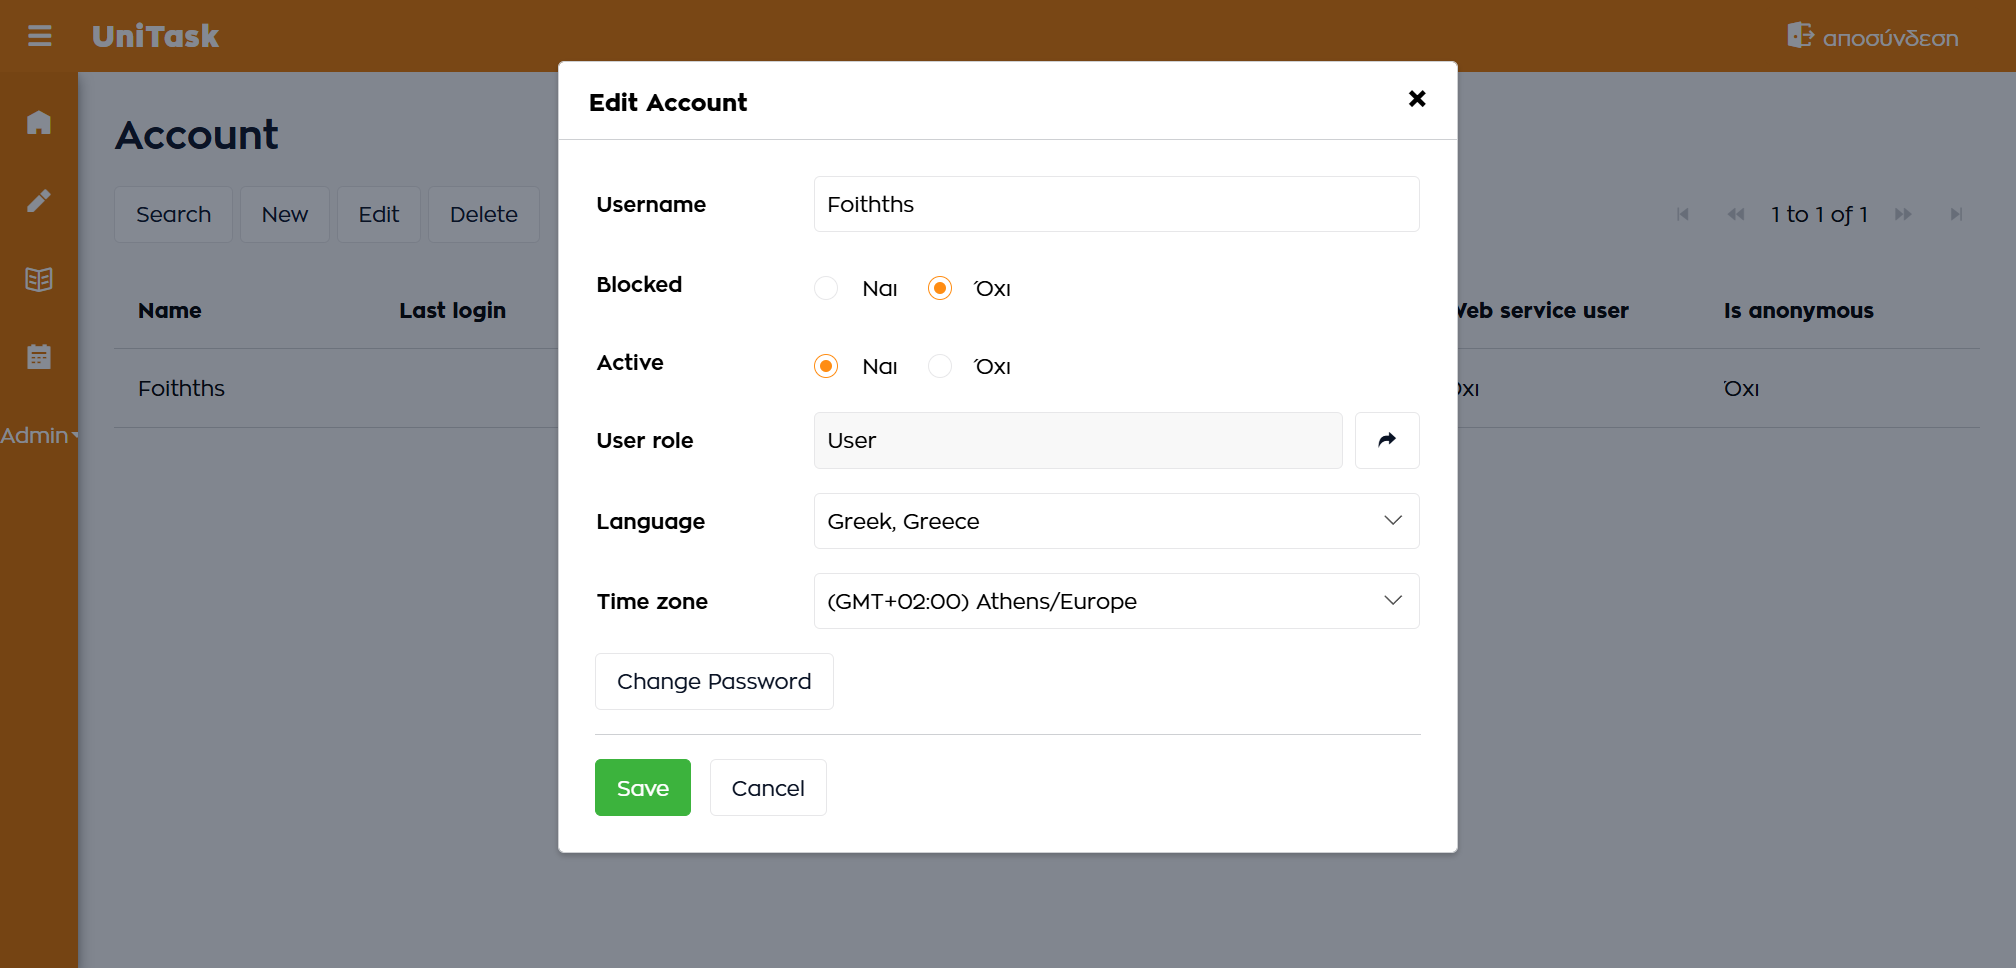
\includegraphics[trim={0 3cm 0 0}, clip, width=\textwidth]{UniTask/EditAccount}
            \caption{\centering Επεξεργασία στοιχείων χρήστη}
            \label{fig:unitask_EditAccount}
        \end{figure}

        \begin{figure}[h!] \noindent \centering
            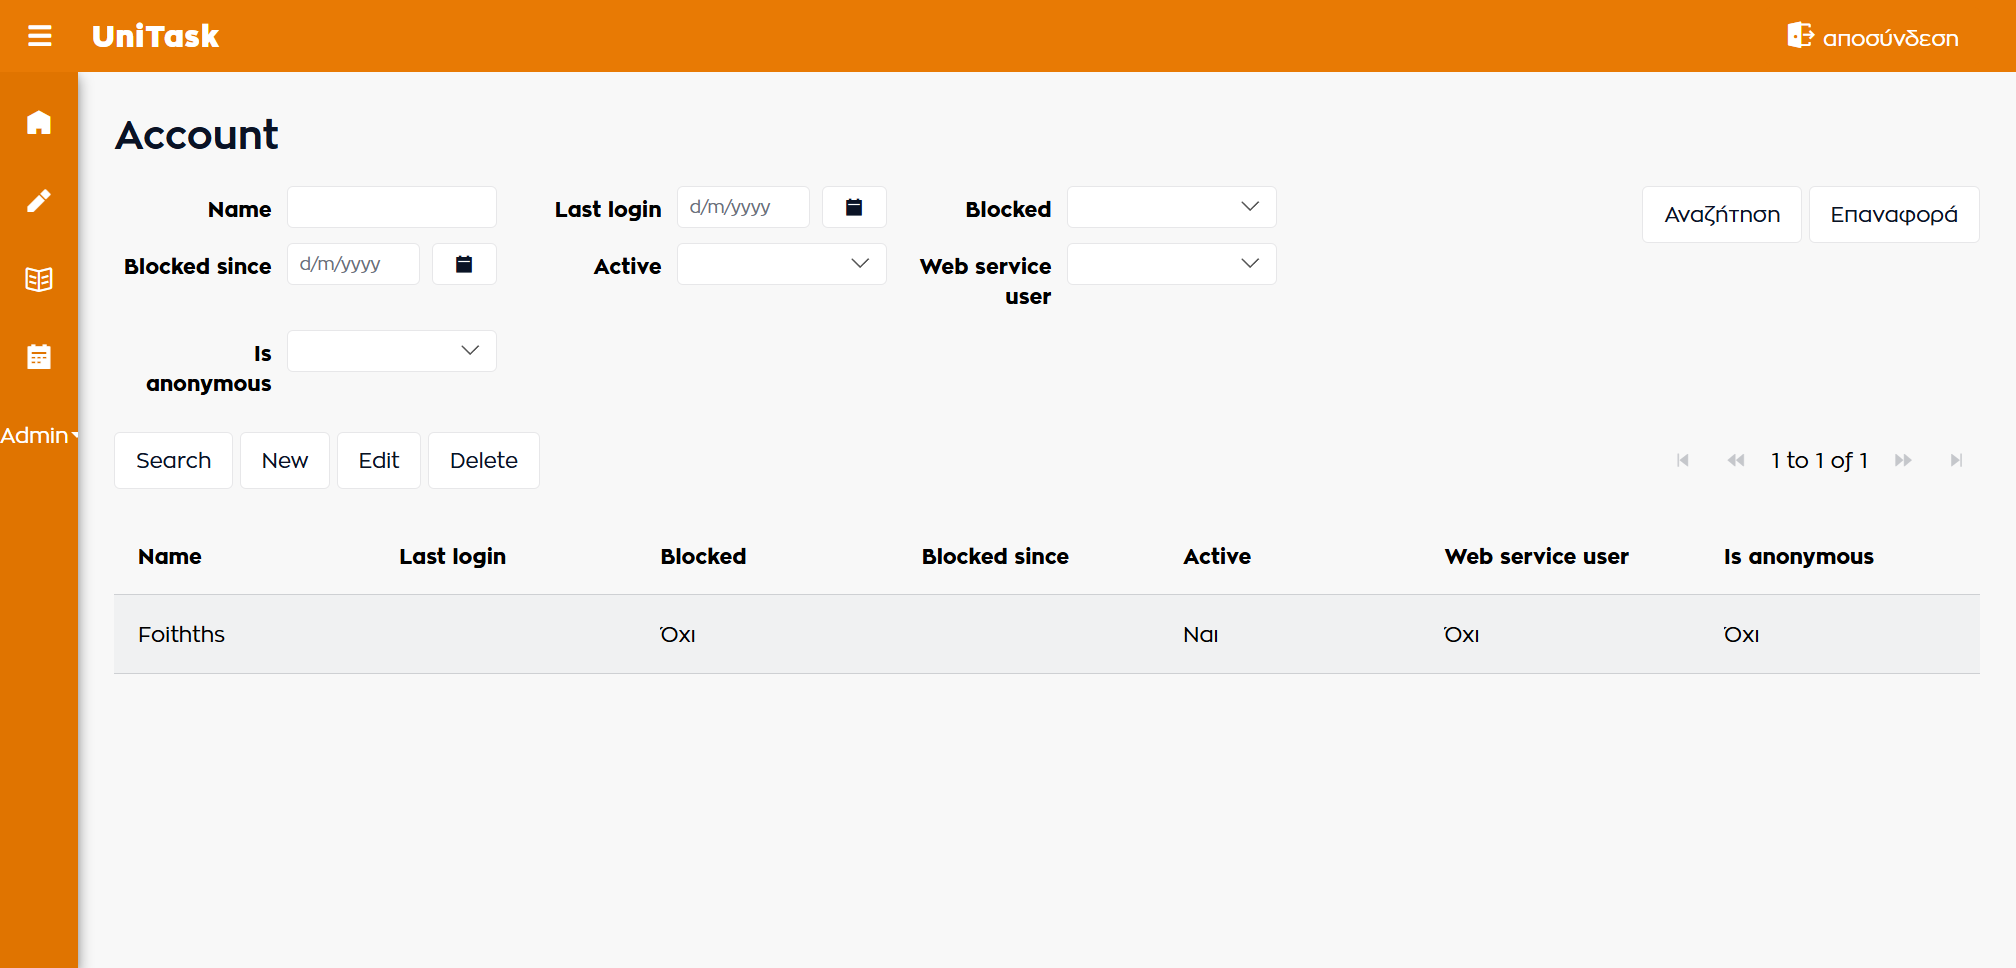
\includegraphics[trim={0 7cm 0 0}, clip, width=\textwidth]{UniTask/SearchAccounts}
            \caption{\centering Αναζήτηση χρήστη}
            \label{fig:unitask_SearchAccounts}
        \end{figure}

    \subsection{Διαχείριση χρηστών}
        Αφού αποσυνδεθούμε και συνδεθούμε ως \texttt{Foithths}, μας υποδέχεται η \textbf{αρχική σελίδα} της εφαρμογής (σχήμα \ref{fig:unitask_Home}). Η σελίδα περιλαμβάνει ένα κεντρικό call to action κουμπί ({\Zona όλες οι εργασίες}) το οποίο οδηγεί στο {\Zona dashboard}.

        \begin{figure}[h!] \noindent \centering
            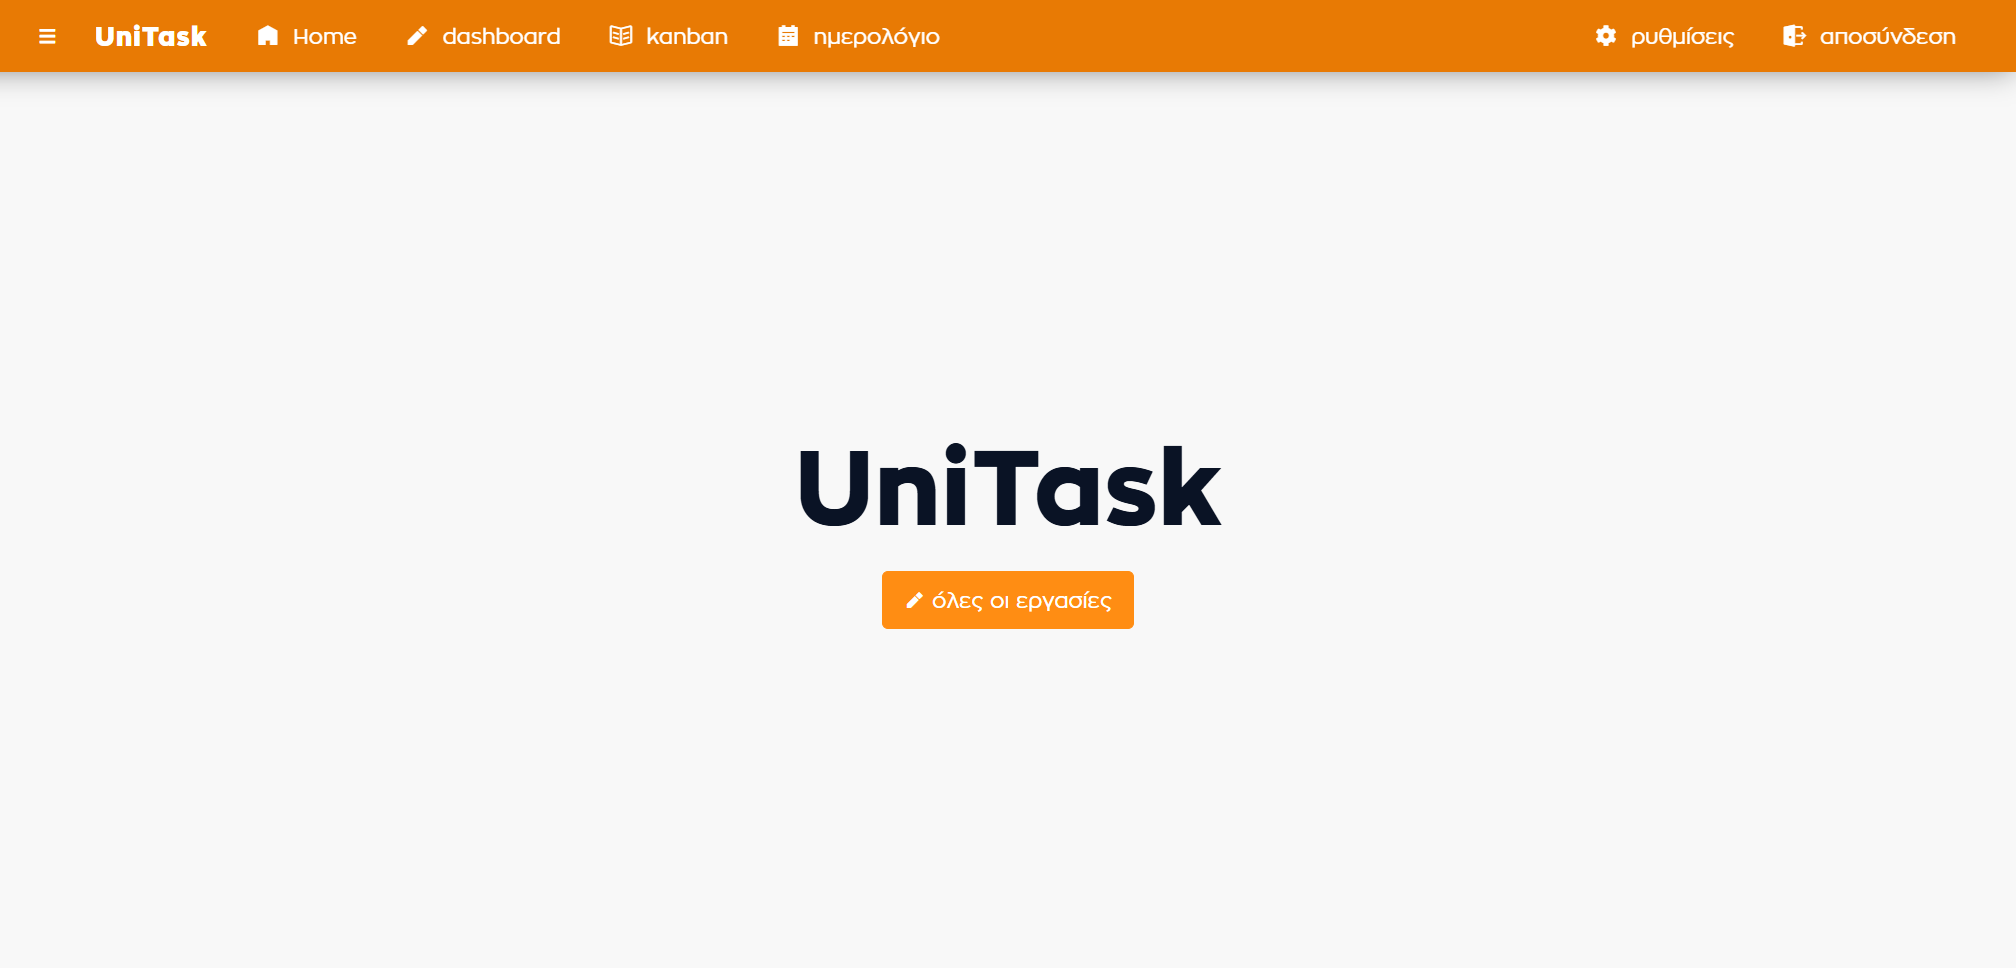
\includegraphics[width=\textwidth]{UniTask/Home}
            \caption{\centering Αρχική σελίδα εφαρμογής}
            \label{fig:unitask_Home}
        \end{figure}

        \begin{figure}[h!] \noindent \centering
            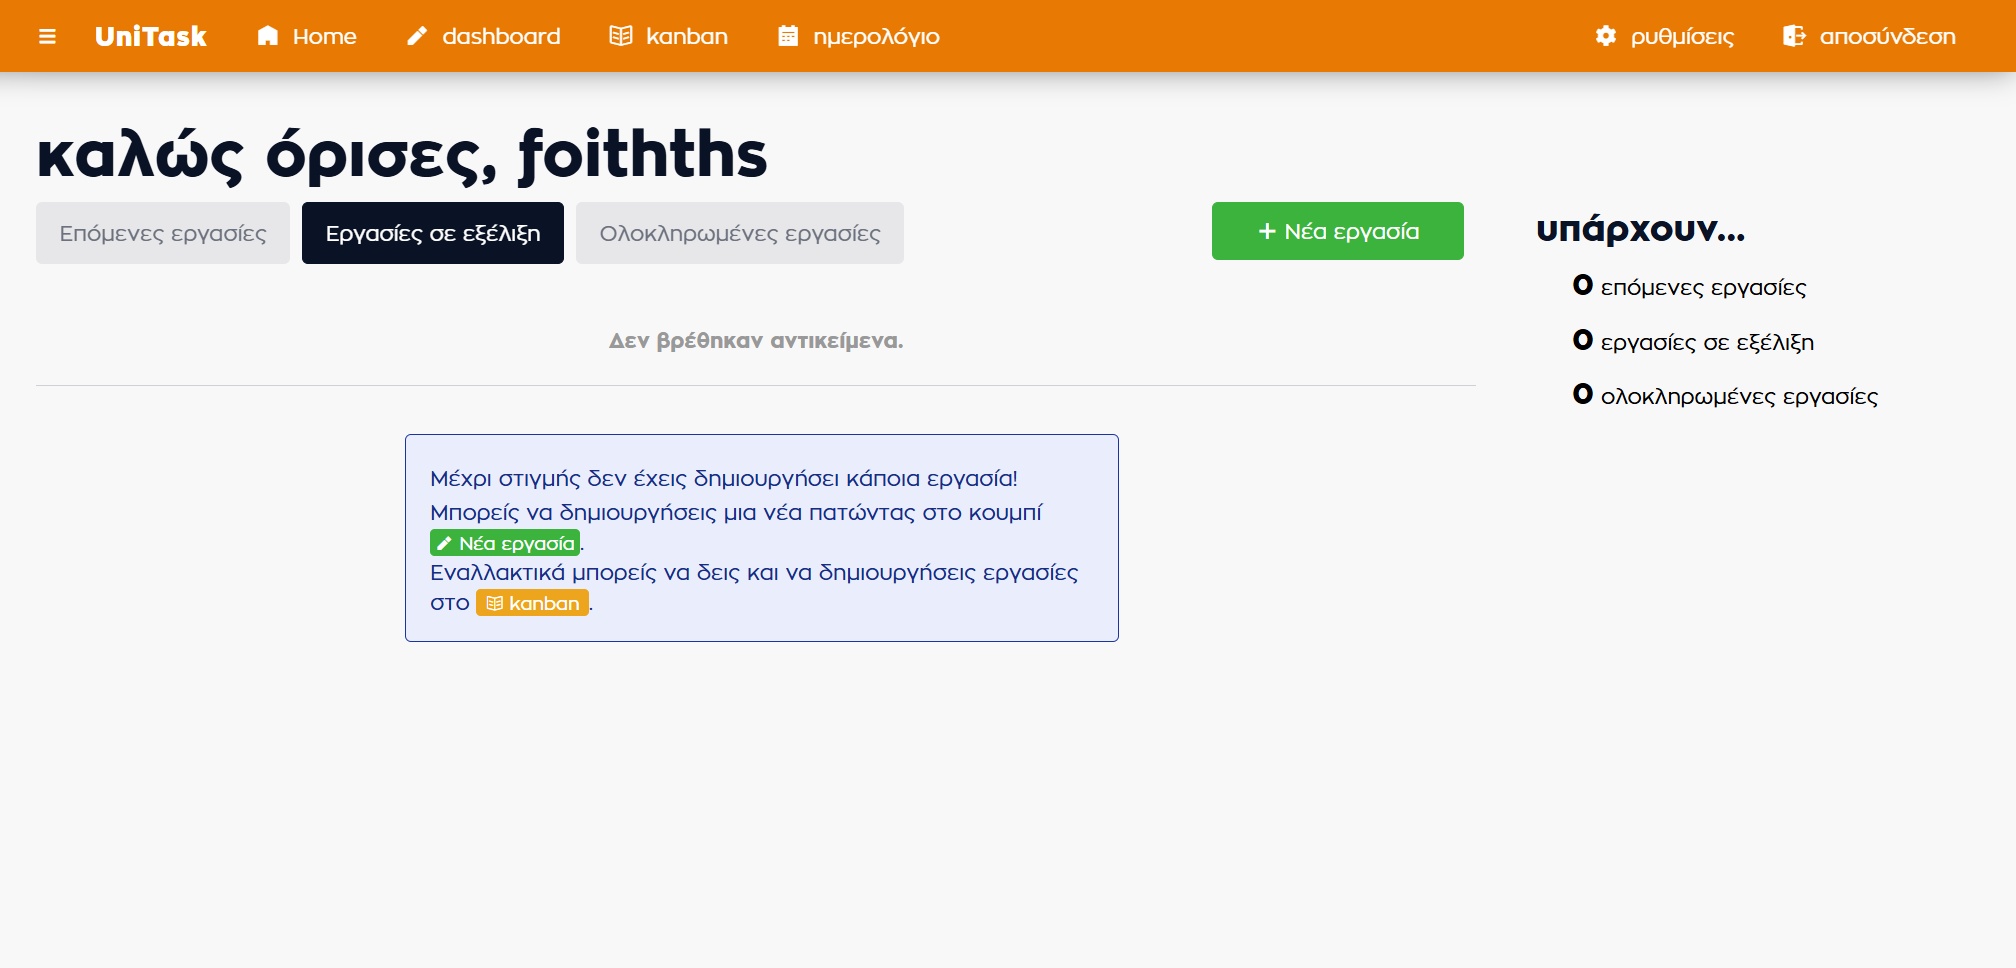
\includegraphics[width=\textwidth]{UniTask/TaskDashboard}
            \caption{\centering Dashboard εργασιών}
            \label{fig:unitask_TaskDashboard}
        \end{figure}

        Στο σχήμα \ref{fig:unitask_TaskDashboard} εμφανίζεται η σελίδα {\ZonaSB dashboard}. Πρόκειται για την κεντρική σελίδα προβολής, δημιουργίας και επεξεργασίας των εργασιών του χρήστη. Περιλαμβάνονται τρεις καρτέλες ({\Zona Επόμενες εργασίες}, {\Zona Εργασίες σε εξέλιξη}, {\Zona Ολοκληρωμένες εργασίες}). Οι επόμενες εργασίες αφορούν εργασίες που έχουν σκοπό να πραγματοποιηθούν στο άμεσο μέλλον αλλά όχι τη δεδομένη χρονική στιγμή, οι εργασίες σε εξέλιξη αφορούν εργασίες που βρίσκονται σε εξέλιξη και οι ολοκληρωμένες εργασίες αφορούν εργασίες που έχουν ολοκληρωθεί.

        Στη σελίδα επίσης περιλαμβάνεται ένα επεξηγηματικό παράθυρο που εμφανίζεται μόνο όταν ο χρήστης δεν έχει δημιουργήσει κάποια εργασία και του εξηγεί το τρόπο λειτουργίας της εφαρμογής. Στο {\Zona dashboard} επίσης περιλαμβάνονται μετρητές για το σύνολο των εργασιών που υπάρχουν ανά κατηγορία, όπως επίσης και ένα κεντρικό κουμπί δημιουργίας εργασιών ({\Zona Νέα εργασία}).



%    \section{Δομή της εφαρμογής} \label{sec:unitask_mendix}